\chapter{Aplicaciones de Mensajería}

Me voy a centrar en Telegram, Whatsapp y Facebook Chat, Signal y la de apple.

\section{Telegram (MTProto)}

Referencias: \cite{Miculan2021} \cite{WebProto}

\subsection{Descripción general}
MTProto 2.0 es una suite de protocolos criptográficos diseñados para implementar de manera rápida, escalable y segura intercambio de mensajes sin depositar esa responsabilidad en la seguridad del transporte debajo de dicho protocolo.
El protocolo esta subdividido en tres componentes virtuales independiente:
\begin{itemize}
	\item \textbf{Componente de alto nivel:} Define el método por el cual las consultas de la API y las respuestas se convierten en mensajes binarios. 
	\item \textbf{Capa criptográfica(autorización):} Define el método por el cual los mensajes están cifrados antes de ser enviados a través del protocolo de transporte.
	\item \textbf{Componente de transporte:} Define el método por el cual el cliente y el servidor para transmitir los mensajes sobre otro protocolo de red como HTTP, HTTPS, WS, WSS, TCP o UDP.
\end{itemize}

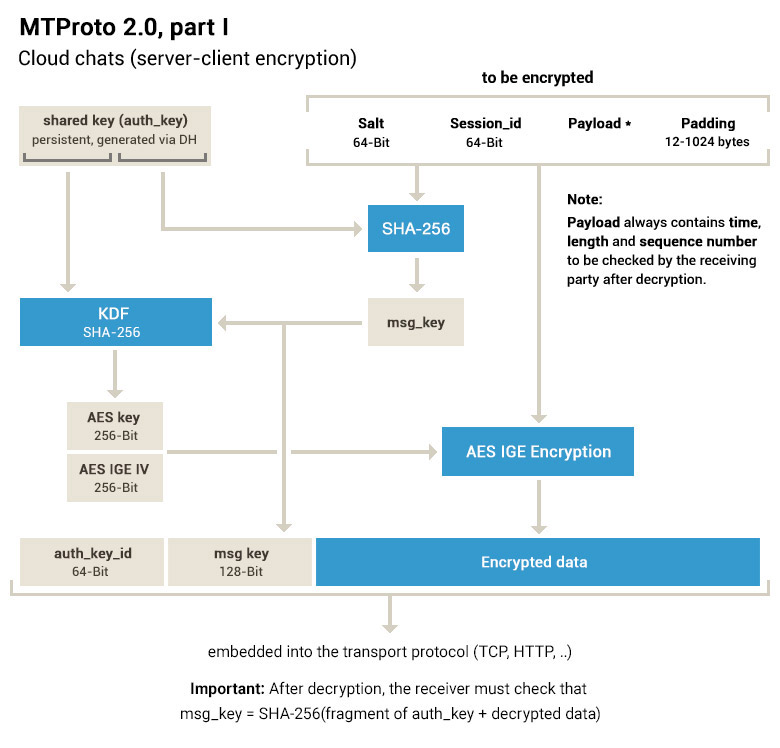
\includegraphics[scale=0.4]{imagenes/diagramaMTProto.jpg} 

\subsection{Resumen de los componentes}
\begin{description}
	\item \textbf{Componentes de alto nivel(Lenguajes de consulta/API RPC):}\\
Desde el punto de vista del componente de alto nivel, el cliente y el servidor intercambian mensajes dentro de una sesión.\\
La sesión se adjunta al cliente en lugar de una conexión \emph{websocket/http/https/tcp.} 
Además, cada sesión tiene asociada a clave ID de usuario mediante la cual se logra la autorización.\\ 
Pueden estar abiertas varias conexiones a un servidor, los mensajes pueden ser enviados en cualquier dirección a través de cualquiera de las conexiones.
Cuando se usa el protocolo UDP, una respuesta puede ser devuelta por una dirección de IP distinta.\\
Hay diferentes tipos de mensajes:
\begin{itemize}
		\item \textbf{LLamadas RPC(cliente-servidor):} LLamadas a los métodos de la API.
		\item \textbf{Respuestas RPC(servidor-cliente):} Resultados de las llamadas RPC.
		\item \textbf{Notificación del estado de los mensajes}
		\item \textbf{Consultas de estado de mensaje}
		\item \textbf{Mensaje multiparte o contenedor}
\end{itemize}

	\item \textbf{Autorización y Cifrado:}
	\item \textbf{Sincronización del tiempo:}
\end{description}
\subsection{Modelo de seguridad}
Los protocolos de Telegram se modelan en ProVerif \cite{ProVer}, que es un verificador criptográfico simbólico. Los protocolos y propiedades de seguridad están especificadas en una variante del \emph{$\pi$-cálculo} que es una notación desarrollada por Robin Milner, Joachim Parrow y David Walker, como un avance sobre el cálculo de sistemas comunicantes con el fin de proveer movilidad al modelado concurrente para representar procesos criptográficos y traducirlos en una teoría de Horn. \\
MTProto 2.0 sigue la siguiente regla de reducción

\lstinputlisting[
    caption=Regla Reducción 1,
    label={lst:listing-cpp},
    language=C++,
    style=CodigoC,
    ]{./ejemplos/ejemplo1.cpp}

\subsection{Protocolo MTProto 2.0}
Como se ha mencionado anteriormente MTProto es una suite cliente/servidor diseñada para acceder a servidores MTProto. Esta suite se puede dividir tres componentes principales.

\begin{itemize}
	\item \textbf{API de alto nivel:} Define como las consultas de la API y respuestas de esta son convertidas en mensajes binarios.
	\item \textbf{Componentes criptográficos y de autorización:} Definen como la aplicaciones se autentifican con el servidor y los mensajes son cifrados antes de ser transmitidos a través del protocolo de transporte.	
	\item \textbf{Componente de transporte:} Define como el cliente y el servidor realmente intercambian los mensajes por un protocolo existente como UDP, TCP, HTTP, HTTPS, etc. Cabe a destacar que también los protocolos de conexión inseguros son soportados.
	\item \textbf{Autorización:} Este módulo provee las funcionalidades para la primera autorización del cliente y del servidor. Se ejecuta solo en la primera ejecución de la aplicación.
\end{itemize}
\\
